%%%%%%%%%%%%%%%%%%%%%%%%%%%%%%%%%%%%%%%%%%%%%%%%%%%%%%%%%%%%%%%%%%%%%%%%
\chapter{Closeness Centrality Ranking in Fully-Dynamic Networks}
\label{ch:dyn-topk}
% Labels: exact, dynamic, distance-based, parallel
%%%%%%%%%%%%%%%%%%%%%%%%%%%%%%%%%%%%%%%%%%%%%%%%%%%%%%%%%%%%%%%%%%%%%%%%
% - What it is and why is it important (applications)
% - Naive algorithm unfeasible in large graphs
% - existing approximation algorithms, description
% - top-k: approx do not always provide a good estimation of the ranking
% - Dynamic graphs, approx does not scale, need for dynamic algo

\section{Introduction}
\label{sec:dyn-topk:intro}
%
%Identifying important vertices in a graph is one of the most prominent
%problems in network analysis~\cite{newman2018networks}. For this purpose,
%several centrality measures have been introduced (see
%\Cref{sec:centrality-measures}).
Closeness centrality (see \Cref{sec:prelim-dist-based-centrality}) is among the
oldest and most widely-studied centrality measures. The intuition of closeness is
that information often travels through shortest paths and thus a vertex is
important or influential if its distance to the others is short.
Popular applications that require to identify such highly central vertices are
influence
maximization~\cite{DBLP:journals/toc/KempeKT15,DBLP:journals/isci/ZhaoWLTG17},
facility
location~\cite{DBLP:journals/pe/GkantsidisMS06,DBLP:conf/icde/LiLCCDZ15},
game theory~\cite{holme2006dynamics}, biology~\cite{DBLP:journals/bmcsb/AshtianiSRHWMJ18}
and sociology~\cite{bavelas1950communication}.

Formally, the closeness centrality of a vertex $u$ is defined as the reciprocal of the
average distance from $u$ to the others and computing it exactly requires
a complete exploration of the graph -- \ie a BFS on unweighted graphs or a complete run
of Dijkstra's algorithm on weighted graphs.
Therefore, computing the closeness centrality of every vertex of a graph
requires to solve the APSP problem, which is impractical on large
real-world instances.

\paragraph{Related Work} In practical applications, centrality is often used to
find the top-$k$ most central vertices and the actual computational effort for
this problem can be substantially cheaper than APSP for large real-world
networks~\cite{DBLP:journals/tkdd/BergaminiBCMM19,DBLP:conf/icde/OlsenLH14}.
%
Despite their superior performance in practice, these strategies have the same
asymptotics as APSP. In particular, assuming the Strong Exponential Time
Hypothesis (SETH)~\cite{DBLP:journals/jcss/ImpagliazzoPZ01}, for any
$\epsilon > 0$, no algorithm can compute the vertex with highest closeness
centrality in $\Oh(n^{2 - \epsilon})$ time for sparse graphs and in $\Oh(m^{2 -
\epsilon})$ time for general graphs~\cite{DBLP:conf/soda/AbboudWW16}.

To overcome this limitation,
several approximation techniques were introduced.
Eppstein and Wang's method~\cite{DBLP:journals/jgaa/EppsteinW04}
selects $1 \le k < n$ \emph{pivot} vertices, runs a complete SSSP
from each of them, and estimates the closeness of a vertex $v$
as $\tilde{\clos}(u) := \frac{k (n - 1)}{n}\sum_{i = 1}^k d(u, v_i)$. It is shown that
$1/\tilde{\clos}(u)$ is an unbiased estimator of $1/\clos(u)$, \ie
$\expected{1/\tilde{\clos}(u)} = 1/\clos(u)$.
By choosing $k \in \Theta\roundb{\log(n)/\epsilon^2}$ pivot vertices, the
algorithm is guaranteed to approximate $\clos(u)$ for each $u \in V$ within an
absolute error of $\epsilon\cdot\diam(G)$ with probability at least $1 - 1/n$.
Cohen \etal~\cite{DBLP:conf/cosn/CohenDPW14} refine this approach and present a
3-approximation algorithm for closeness. Chechik
\etal~\cite{DBLP:conf/approx/ChechikCK15}, in turn, propose an algorithm that
approximates closeness centrality either within a fixed relative standard deviation
(\ie the ratio between the standard deviation and the mean)
$\epsilon$ by performing $\Oh(\epsilon^{-2})$ SSSPs, or within a maximum
relative error of $\epsilon$ with probability at most $1 - 1/poly(n)$ by
performing $\Oh(\log(n) / \epsilon^2)$ SSSPs.

Even though these algorithms provide a precise approximation the closeness
centrality scores, they often fail in ranking the top-$k$ most central vertices
exactly. This is not surprising considering the limited discriminative power of
closeness centrality (as we saw in \Cref{sec:prelim-dist-based-centrality}),
especially for complex networks~\cite[Ch. 7]{newman2018networks}. In order
to provide a correct ranking, approximation
algorithms would lose their competitiveness. For example, Bergamini
\etal~\cite{DBLP:journals/tkdd/BergaminiBCMM19} argue that the algorithm by
Chechik \etal~\cite{DBLP:conf/approx/ChechikCK15} would require $\Oh(n^2m)$
time in unweighted graphs.

\paragraph{Motivation}
Many real-world networks undergo continuous changes (see
\Cref{sec:prelim-dynamic-graphs}). Edge insertions and removals may impact the
closeness centrality score of some vertices and recomputing the ranking after
each edge update is not a scalable solution.
%
A more efficient strategy that was shown to achieve promising results on
related
problems~\cite{DBLP:journals/im/BergaminiM16,DBLP:conf/socialcom/GreenMB12,
DBLP:conf/asunam/KasCC13,DBLP:conf/wea/BergaminiMOS17}
is to exploit previously computed information to update the ranking of the
top-$k$ most central vertices more efficiently in practice than a static
recomputation.

\paragraph{Contribution}
In this chapter, we present new dynamic algorithms for top-$k$
closeness centrality ranking in fully-dynamic graphs.
Our algorithms are developed upon the static algorithm by Bergamini
\etal~\cite{DBLP:journals/tkdd/BergaminiBCMM19}: they use the information
computed on an initial run of the static algorithm to efficiently update
the top-$k$ ranking after multiple edge updates.
Further, they are \emph{exact}, meaning that they provide the correct top-$k$
ranking and the exact closeness centrality scores.
%
Because the traditional definition of closeness centrality
(\Cref{eq:def:closeness}, \Cref{sec:prelim-dist-based-centrality}) does not
apply to not strongly connected graphs, our algorithms compute the \emph{harmonic
centrality} (\Cref{eq:def:harmonic}, \Cref{sec:prelim-dist-based-centrality}),
which does not have such a restriction. However, our techniques can be
easily adapted to the traditional closeness centrality as well.

In \Cref{sec:topk-clos-experimental-results}, our experimental evaluation shows
that, compared to a static recomputation, our dynamic algorithms are up to
four orders of magnitude faster for single edge updates and up to two orders
of magnitude faster for batches of 100 edge updates.

\bibnotes{My contributions among those presented in this chapter involve
the re-implementation of all the dynamic algorithms
(the algorithms for single edge updates were rewritten with additional
improvements that avoid to run \bfscut or \bfsbound when not needed), the
extension of the algorithms to batch updates, and carrying out the experiments.
The remaining contributions are joint work with Patrick Bisenius, Elisabetta
Bergamini, and Henning Meyerhenke. A
preliminary \change{version}~\cite{DBLP:conf/alenex/BiseniusBAM18} of this
work was published in the Proceedings of
the \alenex{Twentieth}{2018}. The aforementioned improvements to the dynamic
algorithms for single edge updates, the extension of the dynamic algorithms to
batch updates, and additional experimental results are presented in an extended
version accepted for publication as a chapter in the
\enquote{Massive Graph Analytics} book edited by David A. Bader and expected to
be released in February 2022.
Preliminary results were part of Patrick Bisenius's Master Thesis, entitled
\enquote{Computing Top-$k$ Closeness Centrality in Fully-dynamic Graphs}}.

\section{Overview of Algorithms for Closeness Centrality}
%
In this section, we provide an overview of existing algorithms for top-$k$
closeness centrality ranking for both static and dynamic graphs.


\subsection{Static Algorithms}
%
The problem of finding the top-$k$ closeness centrality has been targeted
with heuristics, probabilistic approaches and exact algorithms.
Proposed heuristics~\cite{lim2011online,DBLP:journals/ipl/MerrerST14} are based
on sampling or they exploit the correlation between closeness and degree
centrality.
%
Okamoto \etal~\cite{DBLP:conf/faw/OkamotoCL08} introduced a probabilistic algorithm
to compute the top-$k$ closeness centrality ranking in
$\Oh((k + n^{2/3}\log^{1/3}n)(n\log n + m))$ time on general graphs
with probability at least $1 - 1/n$, which is faster than APSP if $k \in o(n)$.
Their strategy is to approximate the centrality scores of every vertex in the graph
with the algorithm by Eppstein and Wang~\cite{DBLP:journals/jgaa/EppsteinW04}
and then to compute the exact centrality scores for a set of \enquote{promising}
candidate vertices.
%
Olsen \etal~\cite{DBLP:conf/icde/OlsenLH14} presented an exact algorithm that efficiently
finds the top-$k$ ranking by scheduling centrality computations in order to minimize the
running time and by reusing intermediate results.
%
These approaches were outperformed by Bergamini
\etal~\cite{DBLP:journals/tkdd/BergaminiBCMM19} who proposed two functions to compute
exactly the top-$k$ vertices with highest closeness centrality on unweighted
undirected graphs:
\nbcut and \nbbound, optimized for complex and high-diameter networks,
respectively. Since our dynamic algorithms are based on these two functions, we
provide a detailed description of them in \Cref{sec:topk-clos-static}.

\subsection{Dynamic Algorithms}
%
Proposed dynamic algorithms for closeness centrality either maintain the scores
of all vertices or the score of just one vertex. In any case, the main strategy is
to run a static algorithm on the initial graph in order to reduce the
computation after an edge update.

Kas \etal~\cite{DBLP:conf/asunam/KasCC13} extended the dynamic APSP algorithm by
Ramalingam and Reps~\cite{DBLP:journals/tcs/RamalingamR96} to also update the
closeness centrality scores of all the vertices of a graph.
A similar strategy was adopted by Khopkar \etal~\cite{DBLP:journals/snam/KhopkarNNB14}
who developed a partially dynamic APSP algorithm that only handles vertex or edge
insertions; the algorithm was extended to update the closeness and the
betweenness centrality of all the vertices of a graph as well.
However, these methods require to compute -- and store -- all the exact pairwise
distances, resulting in unfeasible time and memory requirements on large networks.

Yen \etal~\cite{DBLP:conf/icdm/YenYC13} overcame this limitation by designing a
data structure that efficiently identifies the vertices whose average distance
to the other vertices changes after an edge update. The data structure takes a
linear amount of memory \wrt the size of the graph but is restricted to
undirected and unweighted graphs.
%
Sariy\"uce
\etal~\cite{DBLP:conf/bigdataconf/SariyuceKSC13,DBLP:journals/pc/SariyuceSKC15,
DBLP:journals/corr/abs-1303-0422}
present further optimizations tailored to complex networks to identify
vertices whose closeness centrality score is unaffected by an edge update and
therefore can be skipped. These optimizations were extended to harmonic
centrality by Putman \etal \cite{DBLP:conf/asunam/PutmanBT19}.
Santos \etal \cite{DBLP:conf/ipps/SantosKMS16} proposed a partially
dynamic algorithm that only handles edge deletions.
The main drawback of the aforementioned dynamic algorithms is that they require
to compute the closeness centrality of every vertex of the initial graph,
which is not practical on large-scale graphs.

Finally, the fully-dynamic algorithm by Ni
\etal~\cite{DBLP:conf/asunam/NiHTC19} address the problem of updating the closeness
centrality of a single vertex under the assumption that all edge updates are
already known.

\section{Static Algorithm for Top-$k$ Closeness Centrality}
\label{sec:topk-clos-static}
%
The \nbcut and \nbbound functions try to reduce the computational cost of
running a complete BFS from each vertex in the graph by exploiting upper bounds
of closeness centrality and lazy evaluation.
More precisely, \nbcut starts a BFS from each vertex $u$ in the graph and
interrupts the BFS as soon as it is certain that $u$ cannot be in the top-$k$ ranking.
Conversely, \nbbound does not attempt to prune BFSs, but it runs complete BFSs from
a limited number of vertices.

\subsection{The \nbcut Algorithm for Complex Networks}
\label{sec:nbcut}
%
Assume that we already computed the exact closeness centrality for at least $k$ vertices
and let $h_k$ be the $k$-th highest closeness centrality. While
running a BFS from a vertex $u$, let $\harmupp(u)$ be an upper bound of
$\harm(u)$. Clearly, if $\harmupp(u) < h_k$, then $u$ cannot be among
the top-$k$ vertices with highest closeness centrality, and thus we can
interrupt the BFS. This possibly pruned BFS is named \bfscut.
In the following, we illustrate how $\harmupp(u)$ is defined.

While running a \bfscut from $u$, assume that we just visited all the vertices
up to distance $i$ and thus all the remaining vertices are at distance
at least $i + 1$. Assuming that all the unvisited vertices are at distance
$i + 1$ would already give us a (rather weak) bound. However, we can make further
observations. Let $N_i(u)$ be the set of vertices at distance exactly
$i$ from $u$ and let $n_i(u)$ be its cardinality; each vertex in $N_{i + 1}(u)$ must
have an (incoming) neighbor in $N_i(u)$, and thus we have that $N_{i + 1}(u)
\subseteq \bigcup_{v \in N_i(u)}
\nout(v)$ -- recall from \Cref{sec:prelim-graphs} that $\nout(v)$ are the
out-neighbors of $v$, \ie $N_1(v)$.
This implies that the number of vertices
at distance $i + 1$ from $u$ is, in directed graphs, at most
$\tilde{n}_{i + 1}(u) := \sum_{v \in N_i(u)} \degout(v)$ and, in undirected graphs,
at most $\tilde{n}_{i + 1}(u) := \sum_{v \in N_i(u)} (\deg(v) - 1)$ -- the latter
holds because we can always discard $v$'s parent in the BFS tree.
The distance from $u$ to all the remaining reachable vertices have to be
at least $i + 2$. These observations are summarized in the following bound
on $\harm(u)$:

\begin{equation}
\label{eq:nbcut-bound}
\harmupp(u) := \sum_{v \text{ s.t. } d(u, v) \le i}
\frac{1}{d(u, v)} + \frac{\tilde{n}_{i + 1}(u)}{i + 1} +
\frac{r(u) - \sum_{j = 1}^i n_j(u) - \tilde{n}_{i + 1}(u)}{i + 2}.
\end{equation}

\begin{figure}[tb]
\centering
\begin{tikzpicture}
\footnotesize
\draw[] (0, 0) rectangle (4, 1);
\draw[] (0, 1) -- (2, 5) -- (4, 1) -- cycle;

\coordinate (a) at (intersection of {0,1 -- 2,5} and {0,2 -- 4,2});
\coordinate (b) at (intersection of {2,5 -- 4,1} and {0,2 -- 4,2});
\draw[] (a) -- (b);

\coordinate (a1) at (intersection of {0,1 -- 2,5} and {0,1.5 -- 4,1.5});
\dedge{a}{a1}
\coordinate [below=.5cm of a] (a2);
\dedge{a}{a2}

\coordinate (b1) at (intersection of {2,5 -- 4,1} and {0,1.5 -- 4,1.5});
\dedge{b}{b1}
\coordinate [below=.5cm of b] (b2);
\dedge{b}{b2}

\coordinate (c) at (2, 2);
\coordinate [below left=.5cm and .2cm of c] (c1);
\coordinate [below=.5cm of c] (c2);
\coordinate [below right=.5cm and .2cm of c] (c3);
\dedge{c}{c1}
\dedge{c}{c2}
\dedge{c}{c3}

\coordinate (d) at ($(a)!0.5!(c)$);
\coordinate [below left=.5cm and .2cm of d] (d1);
\coordinate [below right=.5cm and .2cm of d] (d2);
\dedge{d}{d1}
\dedge{d}{d2}

\coordinate (e) at ($(c)!0.5!(b)$);
\coordinate [below left=.5cm and .2cm of e] (e1);
\coordinate [below right=.5cm and .2cm of e] (e2);
\dedge{e}{e1}
\dedge{e}{e2}

\node[] at (2, .5) {$i + 2$};
\node[] at (2, 1.25) {$i + 1$};
\node[] at (2, 3) {Exact};

\filldraw[color=black, fill=white, thick](2,5) circle (.05);
\node[] at (2, 5) [left] {$u$};

\coordinate (x1) at (intersection of {4,2 -- 5,2} and {4.1,0 -- 4.1,5});
\ddedge{4.1, 5}{x1}
\ddedge{x1}{4.1,1}
\ddedge{4.1,1}{4.1,0}

\node[] at (7, 3.5){
$\begin{aligned}
\sum_{v \text{ s.t. } d(u, v) \le i}&\frac{1}{d(u, v)}\\
\end{aligned}$
};

\node[] at (7, 1.5){
$\begin{aligned}
&\frac{\tilde{n}_{i + 1}(u)}{i + 1}
\end{aligned}$
};

\node[] at (7, .5){
$\begin{aligned}
&\frac{r(u) - \sum_{j = 1}^i n_j(u) - \tilde{n}_{i + 1}(u)}{i + 2}
\end{aligned}$
};

\end{tikzpicture}

\caption{Upper bound $\harmupp(u)$ of $\harm(u)$ computed by the \nbcut
algorithm. For all the vertices up to distance $i$ from $u$ we know their
exact distance from $u$. Then, we assume that $\tilde{n}_{i + 1}(u)$ vertices
are at distance $i + 1$ and that the remaining vertices reachable from $u$ are
at distance $i + 2$.}
\label{fig:bfscut}
\end{figure}

As shown in \Cref{fig:bfscut}, the first summand is the contribution to $\harm(u)$
due to the vertices up to distance $i$ from $u$ -- we know their exact distance
from $u$. In the second summand, we assume that $\tilde{n}_{i + 1}(u)$ vertices are
at distance $i + 1$ from $u$\footnote{The numerator can be further tightened
by taking $\min(n - n_i(u), \tilde{n}_{i + 1}(u))$. However, to simplify our notation,
we keep $\tilde{n}_{i + 1}(u)$ in the text, but implement the better bound in practice.}
whereas in the third summand that all the remaining
vertices reachable from $u$ are at distance $i + 2$ from $u$.
%
As $i$ increases the bound tightens: the more \bfscut proceeds the
fewer are the vertices whose distance from $u$ is underestimated.
If $\harmupp(u) < h_k$ for some $i$, then \nbcut interrupts \bfscut
and $\dcut(u) = i$ is called the \emph{cutoff distance} for $u$.
Otherwise, \bfscut is equivalent to a BFS: it visits all the vertices reachable
from $u$ and we have that $\harmupp(u)$ equals $\harm(u)$.

Notice that the third therm of \Cref{eq:nbcut-bound} requires the number of
vertices reachable from any vertex $u$. In undirected graphs, this is the size
of the connected component of $u$ and can be computed in linear time \wrt the
graph size.
In directed graphs, this is the transitive closure, which would be too
expensive to compute. Thus, the authors of
Ref.~\cite{DBLP:journals/tkdd/BergaminiBCMM19} replace $r(u)$ with an upper
bound based on a topological sorting of the SCCs DAG. Furthermore, we observe
that the numerator of the third summand of \Cref{eq:nbcut-bound} cannot be
greater than $n - \sum_{j = 1}^i n_j(u) - \tilde{n}_{i + 1}(u)$. Again, for
simplicity, this detail is omitted in the equation but implemented in practice.

\Cref{algo:nbcut} shows the \nbcut algorithm. Because $h_k$ is not known before
$k$ BFSs are completed, in \Cref{line:nbcut-vk-init} the $k$-th highest
closeness centrality is set to 0. Then, for each vertex $u$ in the graph, the
algorithm starts a \bfscut from $u$ (\Cref{line:nbcut-bfscut}), which returns
the upper bound $\harmupp(u)$ of $u$ and $\texttt{isExact}(u)$, \ie whether
$\harmupp(u)$ equals $\harm(u)$. If \bfscut computes the exact closeness
centrality of $u$, then in
\Crefrange{line:nbcut-update-topk1}{line:nbcut-update-topk2} the algorithm
updates the top-$k$ ranking.
Clearly, \bfscut is more likely to be interrupted if $h_k$ is high.
Hence, ideally, we want to process the vertices by decreasing closeness
centrality. Two promising ordering criteria proposed by the authors
of~\cite{DBLP:journals/tkdd/BergaminiBCMM19} are degree centrality or a measure
based on the number of walks.

\begin{algorithm}[t]
\small
\caption{\small\nbcut algorithm for top-$k$
closeness centrality in static
graphs~\cite{DBLP:journals/tkdd/BergaminiBCMM19}.}
\label{algo:nbcut}
\textbf{Input:} A graph $G = (V, E)$, an integer $1 \le k < n$.\\
\textbf{Output:} Top-$k$ vertices with highest closeness centrality.
\begin{algorithmic}[1]
\State$\topk \gets$ empty min-priority queue with keys $\harm(u)$ and values $u$
\State compute the number of reachable vertices $r(u)$ for each vertex $u \in V$
\State$h_k \gets 0$\label{line:nbcut-vk-init}
\For{\textbf{each} $u \in V$ sorted by an ordering $O$}\label{line:nbcut-for}
\State$\left<\harmupp(u), \isexact(u)\right> \gets \bfscut(u, h_k)$
\label{line:nbcut-bfscut}
\If{$\isexact(u)$ \textbf{and} $\harmupp(u) > h_k$}
\State$\topk.\texttt{push}(\harmupp(u), u)$\label{line:nbcut-update-topk1}
\Comment{Note that here $\harmupp(u) = \harm(u)$}
\If{$\topk.\texttt{size}() > k$}
\State$\topk.\texttt{removeMin}()$
\EndIf
\If{$\topk.\texttt{size}() = k$}
\State$h_k \gets \topk.\texttt{getMinKey}()$\label{line:nbcut-update-topk2}
\EndIf
\EndIf
\EndFor
\State\Return\topk
\end{algorithmic}
\end{algorithm}


\subsection{The \nbbound Algorithm for High-Diameter Networks}
\label{sec:topk-clos-nbbound}
%
\nbbound computes an initial upper bound $\harmupp(u)$ for each vertex $u\in V$,
and stores all the vertices in a max priority queue \prioq
(\Cref{line:nbbound-compute-bound,line:nbbound-prioq-init} of
\Cref{algo:nbbound}). Note that $\harmupp(u)$ is unrelated to the upper bound
$\harmupp(u)$ used by \nbcut described in \Cref{sec:nbcut}, for more details
about $\harmupp(u)$ see~\cite{DBLP:journals/tkdd/BergaminiBCMM19}.
In \Crefrange{line:nbbound-extract}{line:nbbound-early-stop} the algorithm
extracts the vertex $u$ in \prioq with highest $\harmupp(u)$ and terminates
if $\harmupp(u)$ is smaller than the $k$-th largest closeness centrality computed
exactly so far.
%
Otherwise, in \Cref{line:nbbound-bfsbound,line:nbbound-update-pq}
the closeness centrality of $u$ is computed exactly by the \bfsbound
function. \bfsbound might also modify the upper bound of other vertices
in \prioq: assume we are running \bfsbound from $u$ and let $x$ and $y$ be any two
visited vertices; from the triangle inequality if follows that
$d(x, y) \ge |d(u, x) - d(u, y)|$. By assuming that $d(x, y) = |d(u, x) - d(u,
y)|$ for each $x, y \in V$ we obtain an upper bound of the closeness centrality
of all vertices.
If for some vertex $v$ the newly computed upper bound is smaller than their current
one, then $\harmupp(v)$ and \prioq are updated.
Eventually, the \topk ranking is updated
(\Crefrange{line:nbbound-topk-update1}{line:nbbound-topk-update2}).

\begin{algorithm}[tb]
\small
\caption{\small\nbbound algorithm for top-$k$
closeness centrality in static
graphs~\cite{DBLP:journals/tkdd/BergaminiBCMM19}.}
\label{algo:nbbound}
\textbf{Input:} A graph $G = (V, E)$, an integer $1 \le k < n$.\\
\textbf{Output:} Top-$k$ vertices with highest closeness centrality.

\begin{algorithmic}[1]
\State$\topk \gets$ empty min-priority queue with keys $\harm(u)$ and values $u$
\State compute the initial upper bound $\harmupp(u)$ for each $u \in V$
\label{line:nbbound-compute-bound}
\State$\prioq \gets$ max-priority queue with keys $\harmupp(u)$ and values all $u\in V$
\label{line:nbbound-prioq-init}
\While{\prioq is not empty}
\State$u \gets \prioq.\texttt{extractMax}()$\label{line:nbbound-extract}
\If{$\topk.\texttt{size}() = k$ \textbf{and} $\topk.\texttt{getMinKey}() > \harmupp(u)$}
\State\Return\topk\label{line:nbbound-early-stop}
\EndIf
\State$\harm(u) \gets \bfsbound(u)$\label{line:nbbound-bfsbound}
\Comment{Might modify $\harmupp(v)$ for some $v \in \prioq$}
\State Update \prioq according to the new upper bounds\label{line:nbbound-update-pq}
\State$\topk.\texttt{push}(\harm(u), u)$\label{line:nbbound-topk-update1}
\If{$\topk.\texttt{size}() > k$}
\State$\topk.\texttt{removeMin}()$\label{line:nbbound-topk-update2}
\EndIf
\EndWhile
\State\Return\topk
\end{algorithmic}
\end{algorithm}


\section{Dynamic Top-$k$ Closeness Centrality}
%
When an edge is inserted into or removed from the graph, the top-$k$
closeness centrality ranking might change. Our goal is to update the top-$k$ ranking
faster than re-running \nbcut or \nbbound.
In the following, we present new dynamic algorithms to handle single edge updates
and how we generalize them to batches of edge insertions and removals.
We use hereafter the notation for dynamic graphs described in
\Cref{sec:prelim-dynamic-graphs}.

\subsection{Updating the Number of Reachable Vertices}
\label{sec:dyn-topk-update-reachable}
%
Recall that, in \Cref{eq:nbcut-bound}, the upper bound $\harmupp(u)$ computed by \bfscut
requires the number of reachable vertices $r(u)$ or an
upper bound of it.
As mentioned in \Cref{sec:nbcut}, in undirected graphs, this is the number of vertices
in the connected component of $u$. Instead of recomputing the connected component
from scratch after each edge or batch update, we update them with a simple dynamic
algorithm similar to the one presented in~\cite{ediger2013computational}.
Briefly, we compute a spanning forest of the graph. When an edge $(u, v)$
is inserted where $u$ and $v$ belong to different components, we merge the
components and add $(u, v)$ to the forest.
When an edge $(u, v)$ that is part of the forest is removed, we simultaneously run
two BFSs: one from $u$ and one from $v$.
We interrupt the two BFSs as soon as one vertex is explored by both of them. If
$u$ does not reach $v$ anymore, we split the components; otherwise, we add to
the forest the edge connecting $u$'s spanning tree to $v$'s.

In directed graphs, as described in \Cref{sec:nbcut}, we do not compute $r(u)$
exactly but we compute an upper bound of it based on a topological sorting
of the SCCs DAG. Preliminary experiments showed that updating this after each
edge update is the bottleneck of our dynamic algorithm. Hence, we replace
this bound with the number of vertices in the weakly connected component of $u$,
which still represents an upper bound of $r(u)$ and can be updated efficiently
with the same strategy we use for connected components in undirected graphs.


\subsection{Finding Affected Vertices}
\label{sec:dyn-topk-find-affected}
%
Assume that an edge $(u, v)$ is inserted into or removed from a graph $G$.
This could change the closeness centrality of some vertices.
We call such vertices \emph{affected}.
More formally, the set of affected vertices is defined as:
%
\[
A := \set{x \in V : \exists y\in V\ \text{s.t.}\ d'(x, y) \neq d(x, y)}.
\]

Clearly, if $x\in A$, then either $d'(x, u) \neq d(x, u)$ or $d'(x, v) \neq d(x, v)$.
In other words, if the distance between a vertex $x$ and both $u$
and $v$ remains the same after the edge update, then $x$ cannot be affected
because the BFS DAG rooted at $x$ is unchanged.
The set of affected vertices is computed by running two complete BFSs from $u$
and $v$ in $G$ followed by two pruned BFSs from $u$ and $v$ in $G'$ that only
visit the vertices whose distance from $u$ or to $v$ change due to the edge
update -- \ie the affected vertices. In directed graphs, the BFSs from $v$ run
on $G$ transposed and $G'$ since we want to determine the vertices that change
their distance \emph{to} $v$.
A rather obvious optimization is possible when the insertion/removal of an edge
connects/disconnect two (weakly) connected components: in this case we already
know that the affected vertices will be the ones in the two components, and thus
we only need to run two BFSs -- one from $u$ and one from $v$ -- instead of four.


\subsection{Update After an Edge Insertion -- Based on \nbcut}
\label{sec:topk-clos-single-ins-nbcut}
%
We focus on the \nbcut algorithm first. We assume that, after the initial static
run of \nbcut, the quantities $\dcut(u)$, $\harmupp(u)$, and $\isexact(u)$
are know for every vertex $u\in V$. Further, we assume that the top-$k$ vertices
are stored in a min-priority queue \topk.
A simple strategy to update the top-$k$ vertices after an edge insertion would be
to run \bfscut for every affected vertex. This would already be an
improvement compared to the static algorithm -- unaffected vertices are skipped
-- but further optimizations are possible.

\begin{algorithm}[t!]
\setstretch{1}
\footnotesize
\caption{\footnotesize Dynamic \nbcut algorithm to update the
top-$k$ vertices after an edge insertion.}
\label{algo:nbcut-dyn-ins}
\textbf{Input:} A graph $G = (V, E)$, an edge $(u,v) \notin E$, \topk.\\
\textbf{Output:} Top-$k$ vertices with highest closeness centrality in $G' = (V, E \cup \set{(u, v)})$.

\begin{algorithmic}[1]
\State$\prioq \gets$ empty max-priority queue with keys $\harmupp'(x)$ and values $x$
\State$h_k \gets \topk.\texttt{getMinKey}()$
\State compute $r'(x)$ for each $x \in V$\label{line:nbcut-dyn-ins-init1}
\State$A \gets $ compute the set of affected vertices\label{line:nbcut-dyn-ins-aff}
\State compute $d(u, x), d'(u, x), d(x, v), d'(x, v)$ for each $x\in A$
\label{line:nbcut-dyn-ins-init2}\smallskip

\For{each $x \in A$}\Comment{Compute the new bound $\harmupp'(x)$ for each $x\in A$}
\If{$x\in \topk$}\label{line:nbcut-dyn-ins-remove1}
\State$\topk.\texttt{remove}(x)$\label{line:nbcut-dyn-ins-remove2}
\State$h_k \gets 0$
\EndIf
\State$y \gets u$
\If{$G$ is undirected}
\State$y \gets \argmin_{z \in \set{u, v}}d(x, z)$
\EndIf
\If{\textbf{not} $\isexact(x)$ \textbf{and} $\dcut(x) < d(x, y)$}\label{line:nbcut-dyn-ins-upd1}
\State$\harmupp'(x) \gets \harmupp(x) - \frac{r(x)}{\dcut(x) + 2} + \frac{r'(x)}{\dcut(x) + 2}$
\Comment{$x$ is a far-away vertex}
\label{line:nbcut-dyn-ins-far-away}
\ElsIf{\textbf{not} $\isexact(x)$ \textbf{and} $\dcut(x) = d(x, y)$}
\State$\harmupp'(x) \gets \harmupp(x) - \frac{r(x) - r'(x) + 1}{\dcut(x) + 2}
+ \frac{1}{\dcut(x) + 1}$
\label{line:nbcut-dyn-ins-boundary}
\Comment{$x$ is a boundary vertex}
\Else
\State$\harmupp'(x) \gets \harmupp(x) +
\sum_{i = 1}^{\imax}\frac{1}{i + d(x, y)} \roundb{n_i'(y) - n_i(y)}$
\Comment{Distance-based bound}
\label{line:nbcut-dyn-ins-dist-bound}
\State$\dcut(x) \gets \infty$
\label{line:nbcut-dyn-ins-dist-dcut-infty}
\EndIf
\State$\prioq.\texttt{push}(x)$\label{line:nbcut-dyn-ins-upd2}
\EndFor\smallskip

\While{$\prioq$ is not empty}\label{line:nbcut-dyn-ins-resume1}
\State$x \gets \prioq.\texttt{extractMax}()$
\If{$\harmupp'(x) \ge h_k$}
\State$\left<\harmupp'(x), \isexact(x) \right> \gets \bfscut(x, h_k)$
\Comment{We have to run a new \bfscut from $x$}
\Else\ \textbf{break}\label{line:nbcut-dyn-ins-break}
\EndIf
\If{$\isexact(x)$ \textbf{and} $\harmupp'(x) \ge h_k$}
\State$\topk.\texttt{push}(\harmupp'(x), x)$
\Comment{Note that here $\harmupp'(x) = \harm(x)$}
\EndIf
\If{$\topk.\texttt{size}() > k$}
\State$\topk.\texttt{removeMax}()$
\EndIf
\If{$\topk.\texttt{size}() = k$}
\State$h_k \gets \topk.\texttt{getMinKey}()$
\EndIf
\EndWhile\label{line:nbcut-dyn-ins-resume2}
\State update $\harmupp(x), r(x),$ and $n_i(u)$ to $\harmupp'(x), r'(x),$ and $n_i'(x)$, respectively
for each $x\in V$
\State\Return\topk
\end{algorithmic}
\end{algorithm}


\Cref{algo:nbcut-dyn-ins} shows our dynamic algorithm. In
\Crefrange{line:nbcut-dyn-ins-init1}{line:nbcut-dyn-ins-init2} we compute the number
of vertices reachable after the update and the set $A$ of affected vertices
as described in \Cref{sec:dyn-topk-find-affected,sec:dyn-topk-update-reachable}.
Then, in \Cref{line:nbcut-dyn-ins-remove1,line:nbcut-dyn-ins-remove2},
all the affected top-$k$ vertices are removed from \topk.
In \Crefrange{line:nbcut-dyn-ins-upd1}{line:nbcut-dyn-ins-upd2} we
try to avoid starting a new \bfscut from each affected vertex $x$ by
computing the new bound $\harmupp'(x)$ -- more details below --
and we store $x$ in a max-priority queue \prioq
sorted by $\harmupp'(x)$. Finally, in
\Crefrange{line:nbcut-dyn-ins-resume1}{line:nbcut-dyn-ins-resume2}, we resume the \nbcut
algorithm but only for the affected vertices in \prioq and we interrupt it as soon as it
is certain that \topk contains the exact top-$k$ vertices.
In the following, we illustrate how $\harmupp'(x)$ is computed depending on $\dcut(x)$
and the distance from $x$ to the newly added edge.
If $G$ is undirected, let us assume \wilog that
$d(x, u) < d(x, v)$.\footnote{Recall that, as described in
\Cref{sec:dyn-topk-find-affected}, $d(\cdot, u)$ is known from the computation
of the affected vertices.}

\paragraph{Far-away vertices}
%
Let $x$ be an affected vertex such that the \bfscut rooted at $x$ has been interrupted
at the cutoff distance $\dcut(x)$.
If $d(x, u) > \dcut(x)$ and $r'(x) = r(x)$, then $\harmupp(x)$ is still valid because,
as shown in \Cref{fig:far-away-vertex}, $u$ has not been by visited by the
\bfscut rooted at $x$, and therefore the new edge $(u, v)$ does not affect
$\harmupp(x)$.
If $d(x, u) > \dcut(x)$ but $r'(x) \neq r(x)$ -- \ie the insertion increased the
number of vertices reachable from $x$ -- then in \Cref{eq:nbcut-bound} we simply replace
$r(x)$ with $r'(x)$, and we obtain:
%
\[
\harmupp'(x) = \harmupp(x) - \frac{r(x)}{\dcut(x) + 2} + \frac{r'(x)}{\dcut(x) + 2}.
\]

We call $u$ and $v$ \emph{far-away} vertices \wrt $x$, and they are handled
in \Cref{line:nbcut-dyn-ins-far-away} of \Cref{algo:nbcut-dyn-ins}.

\paragraph{Boundary vertices}
%
If $d(x, u)$ equals $\dcut(x)$, then the bound $\harmupp(x)$ is affected because,
as shown in \Cref{fig:boundary-vertex}, $u \in N_{\dcut(x)}(x)$ and
the (out)-degree of $u$ increases by one. Recall from \Cref{sec:nbcut} that in
directed graphs $\tilde{n}_{i + 1}(x) := \sum_{y \in N_i(x)}\degout(y)$ while in
undirected graphs $\tilde{n}_{i + 1}(x) := \sum_{y \in N_i(x)}(\deg(x) - 1)$.
Hence, the upper bound $\tilde{n}_{\dcut(x) + 1}'(x)$ of the number of
vertices at distance $\dcut(x) + 1$ from $x$ after the insertion equals
$\tilde{n}_{\dcut(x) + 1}(x) + 1$.
We can compute the new bound $\harmupp'(x)$ from the old one as follows:
%
\begin{align*}
\harmupp'(x) - \harmupp(x)
=\ &\frac{\tilde{n}_{\dcut(x) + 1}(x) + 1}{\dcut(x) + 1} +
\frac{r'(u) - \sum_{j = 1}^{\dcut(x)}n_j(x) - \tilde{n}_{\dcut(x) + 1}(x) - 1}{\dcut(x) + 2} - \\
&\frac{\tilde{n}_{\dcut(x) + 1}(x)}{\dcut(x) + 1} -
\frac{r(u) - \sum_{j = 1}^{\dcut(x)}n_j(x) - \tilde{n}_{\dcut(x) + 1}(x)}{\dcut(x) + 2}\\
=\ &\frac{1}{\dcut(x) + 1} + \frac{r'(x) - 1 - r(x)}{\dcut(x) + 2}.
\end{align*}

Vertices such as $u$ are called \emph{boundary} vertices \wrt $x$ and they are
handled in \Cref{line:nbcut-dyn-ins-boundary} of \Cref{algo:nbcut-dyn-ins}.

\paragraph{Distance-based Bounds}
%
Let $x$ be an affected vertex such that $d(x, u) < \dcut(x)$ and
let $y$ be any vertex such that $d'(x, y) < d(x, y)$ -- if $x$ is affected
then such a vertex $y$ has to exist.
Since all new shortest paths from $x$ have to go through $(u, v)$ (and thus
through $u$), we can write $d'(x, y)$ as $d'(x, u) + d'(u, y) = d(x, u) + d'(u, y)$.
This holds because the distance from $x$ to $u$ cannot change as a consequence
of the insertion of $(u, v)$ -- recall our assumption at the beginning of this section
that $d(x, u) < d(x, v)$ if $G$ is undirected.
%
As for $d(x, y)$ before the insertion there are two options: either $u$ was
part of a shortest path from $x$ to $y$, and thus $d(x, y) = d(x, u) + d(u, y)$,
or there was a shortest path from $x$ to $y$ not going through $u$, and therefore
$d(x, y) < d(x, u) + d(u, y)$. In any case, $d(x, y) \le d(x, u) + d(u, y)$.
Putting this together we have that
$\frac{1}{d'(x, y)} - \frac{1}{d(x, y)} \le \frac{1}{d(x, u) + d'(u, y)} -
\frac{1}{d(x, u) + d(u, y)}$ and thus:
%
\begin{equation}
\label{eq:nbcut-dist-based-bound}
\begin{split}
\harm'(x) - \harm(x)
&= \sum_{y \in V}\roundb{\frac{1}{d'(x, y)} - \frac{1}{d(x, y)}}\\
&\le \sum_{y \in V}\roundb{\frac{1}{d(x, u) + d'(u, y)} - \frac{1}{d(x, u) + d(u, y)}}\\
&\le \sum_{i = 1}^{\imax}\frac{1}{i + d(x, u)}(n_i'(u) - n_i(u)),
\end{split}
\end{equation}
%
where \imax is the highest value of $i$ such that $n_i'(u) > n_i(u)$.
\Cref{eq:nbcut-dist-based-bound} implies that, if $\harmupp(x)$ is an upper bound
of $\harm(x)$, then
$\harmupp'(x) := \harmupp(x) +
\sum_{i = 1}^{\imax}\frac{1}{i + d(x, u)}(n_i'(u) - n_i(u))$
is an upper bound of $\harm'(x)$.
The values $(n_i'(u) - n_i(u))$ can easily be computed with two BFSs from $u$:
one in $G$ and one in $G'$ -- we integrate this in the BFSs we run to find
the affected vertices, see \Cref{sec:dyn-topk-find-affected}.
Notice that the computation of the new bound requires
$\imax \in \Oh(\diam(G))$ operations. Since the diameter of complex networks is
very small -- often assumed to be logarithmic in $n$, or
constant~\cite{song2005self,DBLP:journals/corr/cond-mat-9907038}
-- this is much faster than running \bfscut, which takes up to
$\Oh(n + m)$ time.
For each affected vertex $x$ for which $u$ is neither far-away nor boundary,
we compute the new upper bound as in \Cref{eq:nbcut-dist-based-bound} --
\Cref{line:nbcut-dyn-ins-dist-bound} of \Cref{algo:nbcut-dyn-ins}.
In \Cref{line:nbcut-dyn-ins-dist-dcut-infty}, we set $\dcut(x)$ to $\infty$ to
indicate that the new bound $\harmupp'(u)$ is not a result of \nbcut anymore
and thus it should not be used in future to identify far-away or boundary
vertices.

\begin{figure}[tb]
\centering
\begin{subfigure}[t]{.45\textwidth}
\centering
\begin{tikzpicture}
\footnotesize
\draw[] (0, 1) -- (2, 5) -- (4, 1) -- cycle;

\coordinate (a) at (intersection of {0,1 -- 2,5} and {0,2 -- 4,2});
\coordinate (b) at (intersection of {2,5 -- 4,1} and {0,2 -- 4,2});
\draw[] (a) -- (b);

\coordinate (a1) at (intersection of {0,1 -- 2,5} and {0,1.5 -- 4,1.5});
\dedge{a}{a1}
\coordinate [below=.5cm of a] (a2);
\dedge{a}{a2}

\coordinate (b1) at (intersection of {2,5 -- 4,1} and {0,1.5 -- 4,1.5});
\dedge{b}{b1}
\coordinate [below=.5cm of b] (b2);
\dedge{b}{b2}

\coordinate (c) at (2, 2);
\coordinate [below left=.5cm and .2cm of c] (c1);
\coordinate [below=.5cm of c] (c2);
\coordinate [below right=.5cm and .2cm of c] (c3);
\dedge{c}{c1}
\dedge{c}{c2}
\dedge{c}{c3}

\coordinate (d) at ($(a)!0.5!(c)$);
\coordinate [below left=.5cm and .2cm of d] (d1);
\coordinate [below right=.5cm and .2cm of d] (d2);
\dedge{d}{d1}
\dedge{d}{d2}

\coordinate (e) at ($(c)!0.5!(b)$);
\coordinate [below left=.5cm and .2cm of e] (e1);
\coordinate [below right=.5cm and .2cm of e] (e2);
\dedge{e}{e1}
\dedge{e}{e2}

\node[] at (2, 3) {Exact};

\filldraw[color=black, fill=white, thick](2,5) circle (.05);
\node[] at (2, 5) [left] {$x$};

\node[] at (b) [right=1mm] {$\dcut(x)$};

\coordinate (u) at (1.75, 1.25);
\coordinate (v) at (2.25, 1.25);
\node[] at (u) [left] {$u$};
\node[] at (v) [right] {$v$};
\dedgecolor{u}{v}{red}
\filldraw[color=black, fill=white, thick] (u) circle (.05);
\filldraw[color=black, fill=white, thick] (v) circle (.05);

\end{tikzpicture}

\caption{$u$ and $v$ are far-away vertices for $x$.}
\label{fig:far-away-vertex}
\end{subfigure}
%
\begin{subfigure}[t]{.45\textwidth}
\centering
\begin{tikzpicture}
\footnotesize
\draw[] (0, 1) -- (2, 5) -- (4, 1) -- cycle;

\coordinate (a) at (intersection of {0,1 -- 2,5} and {0,2 -- 4,2});
\coordinate (b) at (intersection of {2,5 -- 4,1} and {0,2 -- 4,2});
\draw[] (a) -- (b);

\coordinate (a1) at (intersection of {0,1 -- 2,5} and {0,1.5 -- 4,1.5});
\dedge{a}{a1}
\coordinate [below=.5cm of a] (a2);
\dedge{a}{a2}

\coordinate (b1) at (intersection of {2,5 -- 4,1} and {0,1.5 -- 4,1.5});
\dedge{b}{b1}
\coordinate [below=.5cm of b] (b2);
\dedge{b}{b2}

\coordinate (c) at (2, 2);
\coordinate [below left=.5cm and .2cm of c] (c1);
\coordinate [below=.5cm of c] (c2);
\coordinate [below right=.5cm and .2cm of c] (c3);
\dedge{c}{c1}
\dedge{c}{c2}

\node[] at (c) [above] {$u$};
\node[] at (c3) [below] {$v$};
\dedgecolor{c}{c3}{red}
\filldraw[color=black, fill=white, thick] (c) circle (.05);
\filldraw[color=black, fill=white, thick] (c3) circle (.05);


\coordinate (d) at ($(a)!0.5!(c)$);
\coordinate [below left=.5cm and .2cm of d] (d1);
\coordinate [below right=.5cm and .2cm of d] (d2);
\dedge{d}{d1}
\dedge{d}{d2}

\coordinate (e) at ($(c)!0.5!(b)$);
\coordinate [below left=.5cm and .2cm of e] (e1);
\coordinate [below right=.5cm and .2cm of e] (e2);
\dedge{e}{e1}
\dedge{e}{e2}

\node[] at (2, 3) {Exact};

\filldraw[color=black, fill=white, thick](2,5) circle (.05);
\node[] at (2, 5) [left] {$x$};

\node[] at (b) [right=1mm] {$\dcut(x)$};


\end{tikzpicture}

\caption{$u$ is a boundary vertex for $x$.}
\label{fig:boundary-vertex}
\end{subfigure}
\caption{Example of far-away (left) and boundary (right) vertices.}
\label{fig:far-away-boundary}
\end{figure}

\paragraph{Handling multiple edge insertions -- based on \nbcut}
%
A straightforward strategy to handle multiple edge insertions would be to run
\Cref{algo:nbcut-dyn-ins} for each individual edge insertion, which is
unnecessarily expensive because it recomputes the top-$k$ ranking after each
edge insertion -- we are interested in the top-$k$ ranking after multiple edge
insertions. A more efficient approach is to modify \Cref{algo:nbcut-dyn-ins} so
that it computes all the affected vertices $x \in A$ and their new bounds
$\harmupp'(x)$. The top-$k$ ranking is recomputed only once afterwards.
This can be done as follows: for each edge insertion, we update the bounds
of the affected vertices
(\Crefrange{line:nbcut-dyn-ins-init1}{line:nbcut-dyn-ins-upd2}); then, in
\Cref{line:nbcut-dyn-ins-upd2}, we push $x$ into \prioq only if
$x\notin\prioq$, otherwise, we just update its key. Finally, we recompute the
top-$k$ ranking by running
\Crefrange{line:nbcut-dyn-ins-resume1}{line:nbcut-dyn-ins-resume2}.

\subsection{Update After an Edge Insertion -- Based on \nbbound}
\label{sec:topk-clos-single-ins-nbbound}
%
\Cref{algo:nbbound-dyn-ins} shows the pseudocode of our dynamic algorithm
for single edge insertions based on \nbbound.
Let us assume that \nbbound has been executed on the initial graph. Recall
from \Cref{sec:topk-clos-nbbound} that \nbbound runs complete BFSs until
it finds $k$ vertices whose exact closeness centrality is higher than the upper
bounds on the remaining vertices.
Thus, there is no cutoff distance that we can exploit to identify far-away or
boundary vertices, but we can still make some considerations. First, for
unaffected vertices $x\notin A$, $\harm(x)$ and $\harmupp(x)$ are still valid
and do not need to be changed. Further, the distance-based bounds described
in \Cref{sec:topk-clos-single-ins-nbcut} can be applied to \nbbound as well
(\Cref{line:nbbound-dyn-ins-upd-bound} of \Cref{algo:nbbound-dyn-ins}) and,
if there are vertices whose new bound is higher than the $k$-th highest
closeness centrality value, we run a \bfsbound from them
(\Cref{line:nbbound-dyn-ins-bfsbound}).
Similarly to the static \nbbound, we interrupt the algorithm when there are
no affected vertices $x$ whose upper bound $\harmupp(x)$ is higher than
the $k$-th highest closeness centrality (\Cref{line:nbbound-dyn-ins-early-stop}).

\paragraph{Handling multiple edge insertions -- based on \nbbound}
%
Similarly to the \nbcut case, \Cref{algo:nbbound-dyn-ins} can be easily
adapted to handle multiple edge insertions:
\Cref{line:nbbound-dyn-ins-init1,line:nbbound-dyn-ins-init2} are executed
for each edge insertion and then
\Crefrange{line:nbbound-dyn-ins-loop}{line:nbbound-dyn-ins-loop-end} are executed
only once.

\begin{algorithm}[tb]
\small
\caption{\small Dynamic \nbbound algorithm to update the
top-$k$ vertices after an edge insertion.}
\label{algo:nbbound-dyn-ins}
\textbf{Input:} A graph $G = (V, E)$, an edge $(u,v) \notin E$, \topk.\\
\textbf{Output:} Top-$k$ vertices with highest harmonic centrality in $G' = (V, E \cup \set{(u, v)})$.
\begin{algorithmic}[1]
\State$\prioq \gets$ empty max-priority queue with keys $\harmupp(x)$ and values $x$
\State$h_k \gets \topk.\texttt{getMinKey}()$
\State$A \gets $ compute the set of affected vertices\label{line:nbbound-dyn-ins-init1}
\State compute $d(u, x), d'(u, x), d(x, v), d'(x, v)$ for each $x\in A$
\label{line:nbbound-dyn-ins-init2}\smallskip

\For{each $x \in A$}\Comment{Compute the new bound $\harmupp'(x)$ for each $x\in A$}
\label{line:nbbound-dyn-ins-loop}
\If{$x\in \topk$}
\State$\topk.\texttt{remove}(x)$
\State$h_k \gets 0$
\EndIf
\State$y \gets u$
\If{$G$ is undirected}
\State$y \gets \argmin_{z \in \set{u, v}}d(x, z)$
\EndIf
\TopComment{update the bounds of the affected vertices}
\State$\harmupp'(x) \gets \harmupp(x) +
\sum_{i = 1}^{\imax}\frac{1}{i + d(x, y)}(n_i'(y) - n_i(y))$
\label{line:nbbound-dyn-ins-upd-bound}
\State$\prioq.\texttt{push}(\harmupp'(x), x)$\smallskip
\EndFor

\While{$\prioq$ is not empty}\label{line:nbbound-dyn-ins-resume1}
\State$x \gets \prioq.\texttt{extractMax}()$
\If{$\topk.\texttt{size}() = k$ \textbf{and} $\harmupp(x) < h_k$}
\State\Return\topk\label{line:nbbound-dyn-ins-early-stop}
\EndIf
\State$\harm(x) \gets \bfsbound(x)$\label{line:nbbound-dyn-ins-bfsbound}
\Comment{Might modify $\harmupp(z)$ for some $z\in\prioq$}
\State Update \prioq according to the new upper bounds
\State$\topk.\texttt{push}(\harm(x), x)$
\If{$\topk.\texttt{size}() > k$}
\State$\topk.\texttt{removeMin}()$
\EndIf
\EndWhile
\State\Return\topk
\label{line:nbbound-dyn-ins-loop-end}
\end{algorithmic}
\end{algorithm}


\subsection{Update After an Edge Removal}
\label{sec:topk-clos-single-rem}
%
Edge removals are, in some sense, easier to handle than edge insertions:
closeness centrality can only decrease as a consequence of a removal --
distances can only increase -- and thus nothing needs to be done if none of the
top-$k$ vertices are affected. For edge insertions, in turn, there could be
some vertex that increases its closeness centrality and \enquote{overtakes} the
previous $k$-th highest closeness centrality. Further, for an affected vertex
$x$, its previous upper bound $\harmupp(x)$ is still valid -- although it might
be less tight.

\Cref{algo:nbcut-dyn-rem} shows our dynamic algorithm for single edge
removals based on \nbcut.
If we know the exact $\harm(x)$ of an affected vertex $x$ before
the removal, this becomes an upper bound on the closeness centrality of $x$ in
$G'$; then, we set $\isexact(x)$ to \false and, if $x\in\topk$, we remove it
from \topk (\Crefrange{line:nbcut-dyn-rem-aff1}{line:nbcut-dyn-rem-aff2}).
%
Once this is done, the algorithm processes the vertices in the max-priority
queue \prioq sorted by $\harmupp(x)$ and terminates when \topk contains $k$
vertices and the highest $\harmupp(x) \in \prioq$ is smaller than the $k$-th
highest closeness centrality (\Cref{line:nbcut-dyn-rem-early-stop}).
Note that this strategy works for both \nbcut and \nbbound, with the only difference
that, in \Cref{line:nbcut-dyn-rem-bfscut}, we either run \bfscut or \bfsbound.

\begin{algorithm}[tb]
\small
\setstretch{1}
\caption{\footnotesize Dynamic \nbcut algorithm to update the
top-$k$ vertices after an edge removal.}
\label{algo:nbcut-dyn-rem}
\textbf{Input:} A graph $G = (V, E)$, an edge $(u,v) \in E$, \topk.\\
\textbf{Output:} Top-$k$ vertices with highest closeness centrality in
$G' = (V, E \setminus \set{(u, v)})$.

\begin{algorithmic}[1]
\State$h_k \gets \topk.\texttt{getMinKey}()$
\State compute $r'(x)$ for each $x \in V$\label{line:nbcut-dyn-rem-reach}
\State$A \gets $ compute the set of affected vertices
\State compute $d(u, x), d'(u, x), d(x, v), d'(x, v)$ for each $x\in A$
\smallskip

\For{each $x \in A$}
\State$\isexact(x) \gets \false$\label{line:nbcut-dyn-rem-aff1}
\If{$x \in \topk$}
\State$\topk.\texttt{remove}(x)$\label{line:nbcut-dyn-rem-aff2}
\State$h_k \gets 0$\label{line:nbcut-dyn-rem-hk}
\EndIf
\EndFor

\State$\prioq \gets$ max-priority queue with keys $\harmupp'(x)$ and values all
$x\in V \setminus \topk$\label{line:nbcut-dyn-rem-pq}\smallskip

\While{$\prioq$ is not empty}
\State$x \gets \prioq.\texttt{extractMax}()$
\If{$\harmupp(x) < h_k$}
\State\textbf{break}\label{line:nbcut-dyn-rem-early-stop}
\EndIf
\If{\textbf{not} $\isexact(x)$}
\TopComment{we run a new \bfscut from $x$}
\State$\left< \harmupp'(x), \isexact(x) \right> \gets \bfscut(x, h_k)$
\label{line:nbcut-dyn-rem-bfscut}
\EndIf
\If{$\isexact(x)$ \textbf{and} $\harmupp'(x) > h_k$}
\State$\topk.\texttt{push}(\harmupp'(x), x)$
\Comment{Note that here $\harmupp(x) = \harm(x)$}
\EndIf
\If{$\topk.\texttt{size}() > k$}
\State$\topk.\texttt{removeMin}()$
\EndIf
\If{$\topk.\texttt{size}() = k$}
\State$h_k \gets \topk.\texttt{getMinKey}()$
\EndIf
\EndWhile
\State update $\harmupp(x), r(x),$ and $n_i(u)$ to $\harmupp'(x), r'(x),$ and $n_i'(x)$, respectively
for each $x\in V$
\State\Return\topk\label{line:nbcut-dyn-rem-end}
\end{algorithmic}
\end{algorithm}


\paragraph{Handling multiple edge removals}
%
As with multiple edge insertions, multiple edge removals are handled in two
steps. First, all the affected vertices are computed by executing
\Crefrange{line:nbcut-dyn-rem-reach}{line:nbcut-dyn-rem-hk} for each edge
removal. Then, the top-$k$ ranking is updated by running Lines
\Crefrange{line:nbcut-dyn-rem-pq}{line:nbcut-dyn-rem-end} only once.


\subsection{Time Complexity and Memory Requirements}
%
Updating the number of reachable vertices described in
\Cref{sec:dyn-topk-update-reachable} and computing the set of affected vertices
take $\Oh(n + m)$ time in the worst case (the time complexity of a complete
BFS). Then, the algorithms described in
\Cref{sec:topk-clos-single-ins-nbcut,sec:topk-clos-single-ins-nbbound,sec:topk-clos-single-rem}
have to run, in the worst case, one \bfscut (or
\bfsbound, if we are considering the algorithm based on \bfsbound) for each
affected vertex. Since worst-case time complexity of both \bfscut and \bfsbound
is $\Oh(n + m)$~\cite{DBLP:journals/tkdd/BergaminiBCMM19}, the running time of
our dynamic algorithms is $\Oh(|A|(n + m))$ in the worst case, where $|A|$ is
the number of affected vertices. However, as shown in
\Cref{sec:topk-clos-experimental-results}, in real-world networks the actual
number of calls to \bfscut is usually a small fraction of the total number of
affected vertices -- which is, in turn, often only a small fraction of the total
number of vertices.

Concerning memory requirements, for each vertex $u \in V$ our algorithms need
to store the bound $\harmupp(u)$, $\isexact(u)$, the number of reachable vertices
$r(u)$, the cutoff distance $\dcut(u)$, and the \topk priority queue with the
$k$ vertices with highest closeness centrality. This takes only $\Theta(n)$ memory,
which is asymptotically the same as the static top-$k$ algorithms.

\section{Experimental Results}
\label{sec:topk-clos-experimental-results}
%
In this section, we present the results of our experimental study. We study the
impact of the optimizations proposed in \Cref{sec:topk-clos-single-ins-nbcut}
and the algorithmic speedup (ratio between the sequential running times,
see \Cref{sec:prelim-performance-quality}) of our
dynamic algorithms on the static ones.

\subsection{Experimental Setup}
%
We test our algorithms on numerous directed and undirected real-world complex
and high-diameter networks we retrieved from the public repositories
SNAP~\cite{snapnets}, KONECT~\cite{kunegis2013konect},
OpenStreetMap~\cite{OpenStreetMap}, and from
the 9th DIMACS Implementation Challenge~\cite{demetrescu2009shortest}.
The graphs are listed in
\Crefrange{tab:dyn-topk-small-diam-undir}{tab:dyn-topk-high-diam-dir} in
\Cref{sec:dyn-topk-insts}.
%
For high-diameter networks, we only test road networks because they can be
retrieved easily from public repositories, but we are confident that our
dynamic algorithms can handle other types of high-diameter networks as well
without significant difference in performance. To test more undirected
networks, we read as undirected three of the directed road networks
(\enquote{seychelles}, \enquote{comores}, and \enquote{liechtenstein}) by
ignoring the direction of the edges.

For each tested graph, we either add or remove 100 batches of edges selected
uniformly at random and then run both the static and the dynamic algorithms.
For edge insertions, we remove from the original graph an equivalent number of edges
selected uniformly at random before running the algorithms and then we add them
one-by-one, whereas for removals we just remove edges uniformly at random.
Due to time constraints, we only run the static algorithms once every 10 edge
updates -- this does not affect the results considerably, since the running
time of the static algorithms is always approximately the same.

\paragraph{Implementation and settings}
%
Since \nbcut outperforms \nbbound on complex networks, for our experiments on
complex networks we only use \nbcut and our new dynamic algorithms based on it
-- \ie \Cref{algo:nbcut-dyn-ins,algo:nbcut-dyn-rem}.
Similarly, we only use \nbbound (\Cref{algo:nbbound})
and the dynamic algorithms based on it (\Cref{algo:nbbound-dyn-ins}) for our
experiments on road networks.
%
We recall that, for performance reasons, our dynamic algorithms based on \nbcut
for directed graphs use the number of vertices in the WCCs instead of the bound
originally proposed in \cite{DBLP:journals/tkdd/BergaminiBCMM19}. However,
in order to make a fair comparison with previous work, for the static case we
use the original bound.
Further, we recall that all algorithms are \emph{exact}, \ie the find the $k$
vertices with highest closeness centrality and their exact scores, so they only
differ by their running time and not in the results they find.

The machine we use for our experiments is a shared-memory Linux server equipped
with \RAM and an \CPU, of which we use only one because we execute all
algorithms sequentially -- \ie using a single thread.
To ensure reproducibility, all experiments are managed by the SimexPal
software~\cite{DBLP:journals/algorithms/AngrimanGLMNPT19}.
The code has been written in C++ on top of the open-source
NetworKit framework~\cite{DBLP:journals/netsci/StaudtSM16}.


\begin{table}
\footnotesize
\centering
\captionabove{Impact of optimizations in complex networks for $k = 10$,
averaged over 100 batches of 1, 10, 100 random edge insertions using the geometric
mean.
The column \enquote{Aff.} shows the average number of vertices affected by a
single edge insertion, while \enquote{Aff. $(\%)$} the percentage of affected
vertices over the total number of vertices of the graph. The next three columns
report the percentage of affected vertices that are far-away, boundary, or that
are updated using the distance bound. The last column shows the
percentage of affected vertices for which a \bfscut has been run.}
\label{tab:dyn-topk-affected}

\begin{subtable}[t]{\textwidth}
\centering
\caption{Undirected networks}
\label{tab:dyn-topk-affected-undirected}
\begin{tabular}{lrrrrr|rrrr}
\toprule
Network & \multirow{2}{*}{Aff.} & \multirow{2}{*}{Aff. (\%)} &\multirow{2}{*}{F (\%)} & \multirow{2}{*}{B (\%)} & \multirow{2}{*}{D (\%)} & \multicolumn{3}{c}{BFScuts (\%)} \\
Batch size & & & & & & 1 & 10 & 100 \\
\midrule
petster-cat-household & \numprint{3505} & \numprint{3.33} & \numprint{99.45} & \numprint{0.32} & \numprint{0.23} & $<\numprint{0.01}$ & \numprint{0.03} & \numprint{0.22}\\
petster-catdog-household & \numprint{14518} & \numprint{4.36} & \numprint{89.09} & \numprint{10.68} & \numprint{0.23} & $<\numprint{0.01}$ & \numprint{0.04} & \numprint{0.22}\\
petster-cat-friend & \numprint{26} & \numprint{0.01} & \numprint{84.69} & \numprint{14.16} & \numprint{1.15} & $<\numprint{0.01}$ & $<\numprint{0.01}$ & $<\numprint{0.01}$\\
petster-friendships-cat & \numprint{30} & \numprint{0.02} & \numprint{86.89} & \numprint{12.07} & \numprint{1.05} & $<\numprint{0.01}$ & $<\numprint{0.01}$ & $<\numprint{0.01}$\\
petster-friendships-dog & \numprint{1440} & \numprint{0.34} & \numprint{88.76} & \numprint{9.58} & \numprint{1.66} & $<\numprint{0.01}$ & \numprint{0.01} & \numprint{0.17}\\
petster-dog-friend & \numprint{446} & \numprint{0.10} & \numprint{24.59} & \numprint{66.61} & \numprint{8.80} & $<\numprint{0.01}$ & \numprint{0.02} & \numprint{0.17}\\
petster-catdog-friend & \numprint{1620} & \numprint{0.26} & \numprint{92.43} & \numprint{6.37} & \numprint{1.20} & $<\numprint{0.01}$ & $<\numprint{0.01}$ & \numprint{0.15}\\
higgs-twitter-social & \numprint{10342} & \numprint{2.26} & \numprint{84.54} & \numprint{13.59} & \numprint{1.87} & $<\numprint{0.01}$ & \numprint{0.08} & \numprint{1.05}\\
petster-carnivore & \numprint{269} & \numprint{0.04} & \numprint{66.75} & \numprint{27.55} & \numprint{5.70} & $<\numprint{0.01}$ & \numprint{0.02} & \numprint{0.18}\\
\bottomrule
\end{tabular}

\end{subtable}\bigskip

\begin{subtable}[t]{\textwidth}
\centering
\caption{Directed networks}
\label{tab:dyn-topk-affected-directed}

\begin{tabular}{lrrrrr|rrrr}
\toprule
Network & \multirow{2}{*}{Aff.} & \multirow{2}{*}{Aff. (\%)} &\multirow{2}{*}{F (\%)} & \multirow{2}{*}{B (\%)} & \multirow{2}{*}{D (\%)} & \multicolumn{3}{c}{BFScuts (\%)} \\
Batch size & & & & & & 1 & 10 & 100 \\
\midrule
wikipedia\_link\_li & \numprint{2531} & \numprint{5.15} & \numprint{0.10} & \numprint{0.30} & \numprint{99.60} & \numprint{3.51} & \numprint{32.53} & \numprint{94.26}\\
cit-HepPh & \numprint{615} & \numprint{1.78} & \numprint{65.31} & \numprint{4.97} & \numprint{29.73} & \numprint{0.37} & \numprint{3.66} & \numprint{29.08}\\
slashdot-zoo & \numprint{1888} & \numprint{2.39} & \numprint{51.99} & \numprint{11.59} & \numprint{36.43} & \numprint{0.53} & \numprint{7.53} & \numprint{41.64}\\
wiki\_talk\_sv & \numprint{1397} & \numprint{0.23} & \numprint{94.37} & \numprint{5.27} & \numprint{0.36} & $<\numprint{0.01}$ & \numprint{1.16} & \numprint{5.31}\\
munmun\_twitter\_social & \numprint{139} & \numprint{0.03} & \numprint{47.80} & \numprint{20.74} & \numprint{31.46} & $<\numprint{0.01}$ & $<\numprint{0.01}$ & \numprint{0.04}\\
wiki\_talk\_ja & \numprint{1475} & \numprint{0.14} & \numprint{15.98} & \numprint{18.33} & \numprint{65.68} & \numprint{0.05} & \numprint{0.47} & \numprint{2.61}\\
wikipedia\_link\_gu & \numprint{191} & \numprint{0.63} & \numprint{11.43} & \numprint{12.11} & \numprint{76.46} & \numprint{0.47} & \numprint{4.73} & \numprint{25.54}\\
web-NotreDame & \numprint{6332} & \numprint{1.94} & \numprint{91.81} & \numprint{3.33} & \numprint{4.86} & \numprint{0.08} & \numprint{0.36} & \numprint{3.74}\\
digg-friends & \numprint{708} & \numprint{0.02} & \numprint{66.00} & \numprint{18.05} & \numprint{15.95} & $<\numprint{0.01}$ & \numprint{0.03} & \numprint{0.26}\\
\bottomrule
\end{tabular}

\end{subtable}
\end{table}

\subsection{Speedups on Recomputation}
\label{sec:dyn-topk:speedps-rec}
%
\paragraph{Dynamic Complex Networks}
%
\Cref{tab:dyn-topk-affected-undirected} shows the average number of affected
vertices over single edge insertions and the percentage of affected vertices that
are far-away, boundary, or that have been updated using the distance bound
on undirected graphs (results are for $k = 10$).
The average number of affected vertices is at most \maxAffectedPercUndir
of the total number of vertices and for the great
great majority of them $\harmupp'(\cdot)$ can be computed in constant time as they are
either far-away or boundary.
The \enquote{BFScuts} column shows the percentage of
affected vertices from which a new \bfscut is executed after $\harmupp'(\cdot)$ has
been computed for all the affected vertices.
For single edge insertions, our dynamic algorithm always run \bfscut
for less than $\numprint{0.01}\%$ of the number of affected vertices,
while for batches of 10 and 100 edge insertions the number of \bfscut is at most
\maxBFScutsPercUndirBTen and \maxBFScutsPercUndirBHundred the number of vertices
in the graph, respectively.
%
The higher number of \bfscut the batch size can be explained
by the fact that each edge insertion weakens the bounds $\harmupp'(\cdot)$ and thus
reduces the possibility for \Cref{algo:nbcut-dyn-ins} to terminate early at
\Cref{line:nbcut-dyn-ins-break}.

\Cref{tab:dyn-topk-affected-directed} shows the results for the directed case.
Compared to undirected graphs, insertions typically affect smaller portions of
the graph -- average values are at most \maxAffectedPercDir. However, a smaller
percentage of affected vertices is far-away, probably because most of the
vertices that are very close to the inserted edge are affected. Therefore, the
new bounds $\harmupp'(\cdot)$ of the affected vertices are less tight than in the
undirected case and \Cref{algo:nbcut-dyn-ins} runs \bfscut more often -- up to
\maxBFScutsPercDirBOne for single edge insertions and up to
\maxBFScutsPercDirBHundred for batches of 100 edge insertions.

\begin{figure}[tb]
\centering
\begin{subfigure}[t]{\textwidth}
\centering
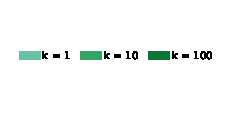
\includegraphics{./sources/plots/dyn-topk/legend-speedup.pdf}
\end{subfigure}\vspace{-20pt}
%
% Complex undirected
%
\begin{subfigure}[t]{.5\textwidth}
\begin{subfigure}[t]{.5\textwidth}
\centering
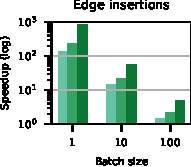
\includegraphics{./sources/plots/dyn-topk/speedup-undirected-small-diameter-addition.pdf}
\end{subfigure}\hfill
\begin{subfigure}[t]{.5\textwidth}
\centering
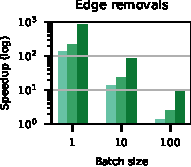
\includegraphics{./sources/plots/dyn-topk/speedup-undirected-small-diameter-removal.pdf}
\end{subfigure}\hfill
\caption{Complex undirected}
\label{fig:dyn-topk-speedup-cmplx-undir}
\end{subfigure}\hfill
%
% Complex directed
%
\begin{subfigure}[t]{.5\textwidth}
\begin{subfigure}[t]{.5\textwidth}
\centering
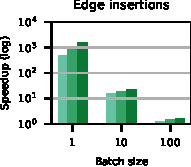
\includegraphics{./sources/plots/dyn-topk/speedup-directed-small-diameter-addition.pdf}
\end{subfigure}\hfill
\begin{subfigure}[t]{.5\textwidth}
\centering
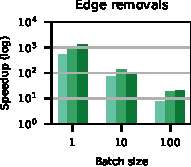
\includegraphics{./sources/plots/dyn-topk/speedup-directed-small-diameter-removal.pdf}
\end{subfigure}\hfill
\caption{Complex directed}
\label{fig:dyn-topk-speedup-cmplx-dir}
\end{subfigure}\medskip

% Road undirected
%
\begin{subfigure}[t]{.5\textwidth}
\begin{subfigure}[t]{.5\textwidth}
\centering
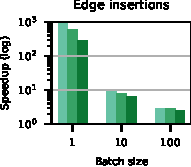
\includegraphics{./sources/plots/dyn-topk/speedup-undirected-high-diameter-addition.pdf}
\end{subfigure}\hfill
\begin{subfigure}[t]{.5\textwidth}
\centering
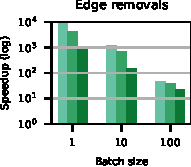
\includegraphics{./sources/plots/dyn-topk/speedup-undirected-high-diameter-removal.pdf}
\end{subfigure}\hfill
\caption{High-diameter undirected}
\label{fig:dyn-topk-speedup-road-undir}
\end{subfigure}\hfill
%
% Complex directed
%
\begin{subfigure}[t]{.5\textwidth}
\begin{subfigure}[t]{.5\textwidth}
\centering
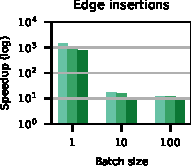
\includegraphics{./sources/plots/dyn-topk/speedup-directed-high-diameter-addition.pdf}
\end{subfigure}\hfill
\begin{subfigure}[t]{.5\textwidth}
\centering
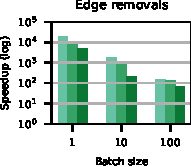
\includegraphics{./sources/plots/dyn-topk/speedup-directed-high-diameter-removal.pdf}
\end{subfigure}\hfill
\caption{High-diameter directed}
\label{fig:dyn-topk-speedup-road-dir}
\end{subfigure}
%
\caption{Geometric mean of the average speedups over all tested networks, for
different values of $k$ and batch sizes.
\Cref{fig:dyn-topk-speedup-cmplx-undir,fig:dyn-topk-speedup-cmplx-dir} show the
results for complex networks, whereas
\Cref{fig:dyn-topk-speedup-road-undir,fig:dyn-topk-speedup-road-dir} show
the results for road networks. Detailed numbers can be found in
\Cref{sec:dyn-topk-add-exp-complex,sec:dyn-topk-add-exp-road}.}
\label{fig:dyn-topk-speedups-summary}
\end{figure}

\begin{figure}[tb]
\centering
\begin{subfigure}[t]{\textwidth}
\centering
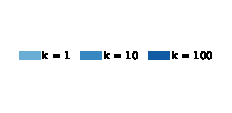
\includegraphics{./sources/plots/dyn-topk/legend-breakdown.pdf}
\end{subfigure}\vspace{-20pt}

% Complex undirected
\begin{subfigure}[t]{.5\textwidth}
\begin{subfigure}[t]{.5\textwidth}
\centering
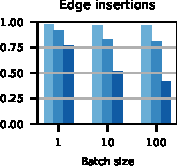
\includegraphics{./sources/plots/dyn-topk/breakdown-undirected-small-diameter-addition.pdf}
\end{subfigure}\hfill
\begin{subfigure}[t]{.5\textwidth}
\centering
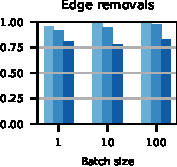
\includegraphics{./sources/plots/dyn-topk/breakdown-undirected-small-diameter-removal.pdf}
\end{subfigure}\hfill
\caption{Complex undirected}
\label{fig:dyn-topk-breakdown-cmplx-undir}
\end{subfigure}\hfill
%
% Complex directed
%
\begin{subfigure}[t]{.5\textwidth}
\begin{subfigure}[t]{.5\textwidth}
\centering
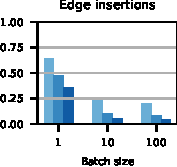
\includegraphics{./sources/plots/dyn-topk/breakdown-directed-small-diameter-addition.pdf}
\end{subfigure}\hfill
\begin{subfigure}[t]{.5\textwidth}
\centering
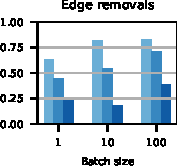
\includegraphics{./sources/plots/dyn-topk/breakdown-directed-small-diameter-removal.pdf}
\end{subfigure}\hfill
\caption{Complex directed}
\label{fig:dyn-topk-breakdown-cmplx-dir}
\end{subfigure}\medskip

% Road undirected
\begin{subfigure}[t]{.5\textwidth}
\begin{subfigure}[t]{.5\textwidth}
\centering
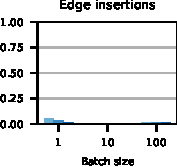
\includegraphics{./sources/plots/dyn-topk/breakdown-undirected-high-diameter-addition.pdf}
\end{subfigure}\hfill
\begin{subfigure}[t]{.5\textwidth}
\centering
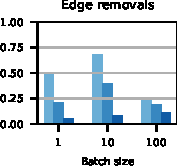
\includegraphics{./sources/plots/dyn-topk/breakdown-undirected-high-diameter-removal.pdf}
\end{subfigure}\hfill
\caption{High diameter undirected}
\label{fig:dyn-topk-breakdown-road-undir}
\end{subfigure}\hfill
%
% Road directed
%
\begin{subfigure}[t]{.5\textwidth}
\begin{subfigure}[t]{.5\textwidth}
\centering
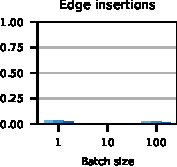
\includegraphics{./sources/plots/dyn-topk/breakdown-directed-high-diameter-addition.pdf}
\end{subfigure}\hfill
\begin{subfigure}[t]{.5\textwidth}
\centering
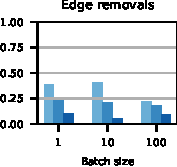
\includegraphics{./sources/plots/dyn-topk/breakdown-directed-high-diameter-removal.pdf}
\end{subfigure}\hfill
\caption{High diameter directed}
\label{fig:dyn-topk-breakdown-road-dir}
\end{subfigure}

\caption{Geometric mean of the average time spent by the dynamic algorithm
computing $\harmupp'(\cdot)$ \wrt the total time spent in updating the top-$k$ nodes
with highest closeness centrality over all the tested networks, for different
values of $k$ and batch sizes.
\Cref{fig:dyn-topk-breakdown-cmplx-undir,fig:dyn-topk-breakdown-cmplx-dir}
show the results for complex networks,
whereas
\Cref{fig:dyn-topk-breakdown-road-undir,fig:dyn-topk-breakdown-road-dir}
show the results for road networks.}
\label{fig:dyn-topk-breakdown}
\end{figure}

\Cref{fig:dyn-topk-speedup-cmplx-undir,fig:dyn-topk-speedup-cmplx-dir}
summarize the speedup of our dynamic algorithm on the static one for complex
networks while \Cref{fig:dyn-topk-breakdown-cmplx-undir,fig:dyn-topk-breakdown-cmplx-dir}
show the fraction of time spent by the dynamic algorithm computing $\harmupp'(\cdot)$ of
the affected vertices \wrt the algorithm's overall running time (\ie computing
$\harmupp'(\cdot)$ and the new top-$k$ ranking) for complex networks.
Detailed results for insertions in complex networks are reported in
\Cref{tab:dyn-topk-speed-ins-cmplx,tab:dyn-topk:time-ins-cmplx}.
%
For undirected networks, the geometric mean of the speedups over 100 single
edge insertions are always at least in the double-digit range for every instance.
Also, the speedups grow for bigger values of $k$, reaching an average speedup (over
all tested undirected instances) of \speedupComplexUndInsertKHundredBOne for
$k = 100$. A possible explanation for this pattern is that separating the top-$k$
vertices with highest closeness centrality from the others is harder for larger
values of $k$ and the dynamic algorithm does this faster because it exploits
precomputed values of $\harmupp'(\cdot)$. This is also clear from the left plot of
\Cref{fig:dyn-topk-breakdown-cmplx-undir}, as updating the ranking becomes more
expensive for larger values of $k$.

For larger batches of edge insertions, our dynamic algorithm yields diminishing
returns. This is expected because, the more the graph changes, the less accurate
the bounds $\harmupp'(\cdot)$ become. As we can clearly see from
\Cref{fig:dyn-topk-breakdown-cmplx-undir}, inaccurate bounds jeopardize the
performance of the dynamic algorithm since the recomputation of the ranking becomes
more expensive as we increase the batch size.
Nevertheless, averaging over all the undirected networks, with $k = 1$ the dynamic
algorithm handles batches of 100 edge insertions
\speedupComplexUndInsertKOneBHundred faster than the static algorithm,
\speedupComplexUndInsertKTenBHundred faster with $k = 10$, and
\speedupComplexUndInsertKHundredBHundred faster with $k = 100$.

Concerning directed graphs, the average speedups for single edge insertions are better
than for the undirected case: the average speedup over all the tested directed
networks are \speedupComplexDirInsertKOneBOne for $k = 1$,
\speedupComplexDirInsertKTenBOne for $k = 10$ and
\speedupComplexDirInsertKHundredBOne for $k = 100$.
%
This can be explained by the smaller number of affected vertices in directed networks
(see \Cref{tab:dyn-topk-affected-directed}). The performance of the dynamic
algorithm for directed networks seems to be more susceptible to the batch
size than for undirected networks; for example, for $k = 10$ and 10 edge insertions,
the average speedup is \speedupComplexDirInsertKTenBTen on
directed networks and \speedupComplexUndInsertKTenBTen on undirected networks,
while for 100 edge insertions the average speedup is
\speedupComplexDirInsertKTenBHundred and \speedupComplexUndInsertKTenBHundred
respectively.
%
Similarly to the undirected case, this is likely due to the inaccuracy of the
updated bounds as the dynamic algorithm spends the vast majority of its running
time in recomputing the ranking (see the left plot in
\Cref{fig:dyn-topk-breakdown-cmplx-dir}).

Speedups for edge removals on complex networks are summarized in the right of
\Cref{fig:dyn-topk-speedup-cmplx-undir,fig:dyn-topk-speedup-cmplx-dir} --
detailed results are reported in
\Cref{tab:dyn-topk-speed-rem-cmplx,tab:dyn-topk:time-rem-cmplx}.
Interestingly, for directed graphs, our algorithm handles removals faster than
insertions, whereas the performance does not change substantially \wrt insertions
in the undirected case. In general, for shortest-path based problems insertions
are easier to handle than removals; for example, pairwise distances can be
updated in $\Oh(n^2)$ time after an edge insertion, but not after an edge
removal~\cite{DBLP:journals/jacm/DemetrescuI04}. In our case, we know that
removals can only \emph{decrease} centrality. Thus, the upper bounds
of the centralities are still valid and, if none of the top-$k$ vertices
is affected, nothing needs to be done.
In insertions, on the contrary, any vertex could \emph{increase} its centrality
and become one of the top-$k$.
If the number of affected vertices is small -- as in most cases for directed graphs,
see \Cref{tab:dyn-topk-affected-directed} -- it is quite unlikely that a top-$k$
vertex is affected. This happens more often in undirected graphs, where often a larger
number of vertices are affected. Consequently, as shown in
\Cref{fig:dyn-topk-breakdown-cmplx-undir,fig:dyn-topk-breakdown-cmplx-dir},
updating the ranking is less expensive after an edge removal than after an edge
insertion.
%
As for insertions, speedups increase with $k$ and decrease with the batch
size: for single edge removals, the geometric mean of the speedups in
undirected graphs is \speedupComplexUndRemovalKOneBOne for $k=1$,
\speedupComplexUndRemovalKTenBOne for $k=10$, and
\speedupComplexUndRemovalKHundredBOne for $k=100$, whereas for directed graphs
it is \speedupComplexDirRemovalKOneBOne for $k=1$,
\speedupComplexDirRemovalKTenBOne for $k=10$, and
\speedupComplexDirRemovalKHundredBOne for $k=100$.
%
For edge removals, the decrease of the speedups \wrt the batch size is less severe
than for edge insertions; the bounds on the
closeness centrality after a batch of edge removals are likely to be tighter than the ones
computed after a batch of edge insertions, allowing \Cref{algo:nbcut-dyn-rem} to terminate
often earlier than \Cref{algo:nbcut-dyn-ins}.


\paragraph{Dynamic Road Networks}
%
\Cref{fig:dyn-topk-speedup-road-undir,fig:dyn-topk-speedup-road-dir} summarize
the speedups for directed and undirected road networks, respectively --
detailed results are shown in
\Cref{tab:dyn-topk-speed-ins-road,tab:dyn-topk-speed-rem-road,tab:dyn-topk:time-ins-road,tab:dyn-topk:time-rem-road} --
whereas
\Cref{fig:dyn-topk-breakdown-road-undir,fig:dyn-topk-breakdown-road-dir} show
the fraction of time spent by the dynamic algorithm updating $\harmupp'(\cdot)$ \wrt
the algorithm's overall running time.
%
As for complex networks, speedups in road networks are generally higher in
the directed case and they decrease with the batch size. However, differently
from complex networks, speedups generally decrease with $k$: If $k$ is large,
it is also more likely that some affected vertices are either among the top-$k$
or \enquote{overtake} one of the top-$k$, making the algorithm run \bfsbound more
often and thus slowing it down. The bar plots in the left of
\Cref{fig:dyn-topk-breakdown-road-undir,fig:dyn-topk-breakdown-road-dir}
also show that the running time of the dynamic algorithm is dominated by the
recomputation of the ranking, which is expected because closeness centrality
distinguishes vertices in complex networks less efficiently than in high-diameter
networks~\cite[Ch. 7]{newman2018networks}.
Nevertheless, even for $k = 100$, for a single edge insertion
the dynamic algorithm is on average \speedupStreetUndInsertKHundredBOne faster than
a static recomputation in undirected road networks
and \speedupStreetDirInsertKHundredBOne faster in directed road networks.
Furthermore, regarding multiple edge insertions, the dynamic
algorithm is faster than a static recomputation on all the considered instances and
for all the considered batch sizes.

Results for removals are significantly better: for $k = 1$ and single edge removals
the dynamic algorithm is on average
\speedupStreetUndRemovalKOneBOne faster in the undirected case and
\speedupStreetDirRemovalKOneBOne in the directed one, while
for $k = 100$ the speedups are \speedupStreetUndRemovalKHundredBOne
and \speedupStreetDirRemovalKHundredBOne, respectively.
%
As we described previously, the impact on the ranking due to edge
removals is in general lower than edge insertions, so the dynamic algorithm
spends less time on recomputing the ranking. This is also clear from the bar
plots in the right of
\Cref{fig:dyn-topk-breakdown-road-undir,fig:dyn-topk-breakdown-road-dir}:
after edge removals the fraction of time spent by the dynamic algorithm
updating $\harmupp'(\cdot)$ \wrt the total running time is greater than after edge
insertions.
%
Finally, concerning batches of 10 [100] edge removals, the dynamic algorithm is
on average two to three [one to two] orders of magnitude faster than a static
recomputation.

\section{Conclusions}
%
In this chapter, we addressed the problem of preserving an exact top-$k$
ranking of the vertices with highest closeness (including their exact score).
We implemented batch-dynamic algorithms for top-$k$
closeness centrality tailored to both complex and high-diameter networks.
Our dynamic algorithms are developed on top of the static algorithms for top-$k$
closeness centrality by Bergamini \etal~\cite{DBLP:journals/tkdd/BergaminiBCMM19};
in particular, they maintain upper bounds $\harmupp(\cdot)$ on the closeness
centrality of every vertex, which accelerates the computation of the top-$k$
vertices in practice.
By re-using such bounds as well as other precomputed information, we are able
to significantly reduce the number of operations required to update the most
central vertices in the graph after multiple graph updates.

As a result, for single edge updates, we achieve high speedups \change{on a}
static recomputation, in line with results obtained by other dynamic algorithms
for related
problems~\cite{DBLP:journals/im/BergaminiM16,DBLP:conf/wea/BergaminiMOS17,
DBLP:conf/socialcom/GreenMB12,DBLP:conf/asunam/KasCC13} -- confirming that
efforts in developing dynamic algorithms are well spent.
%
As we increase the batch sizes, our strategy yield\change{s} diminishing
returns. This is expected because, the more the graph changes, the less precise
the upper bounds $\harmupp'(\cdot)$ become and this impacts the performance of
our dynamic algorithms. Nevertheless, experimental data show that, averaging
results over the tested instances, our dynamic algorithms are always faster
than a static recomputation. \change{In contrast to} most existing algorithms
for updating shortest-path based centralities \change{that require $\Oh(n^2)$
additional memory,} the techniques we propose require an
amount of memory that is \change{only} linear in $n$. Although storing more data
(\eg the distances computed during \bfscut on the initial graph) might lead to
even higher speedups, a quadratic memory footprint would not allow us to target
networks with millions of vertices. An interesting question is whether the
memory requirements of other dynamic algorithms for related problems can be
reduced by using techniques similar to the ones we presented in this chapter.

A possible direction for future research is the extension of our strategies
for batch updates to other centrality
measures such as betweenness -- for which a static algorithm for finding the
top-$k$ vertices with highest betweenness has already been proposed in
Ref.~\cite{DBLP:conf/www/LeeC14}. Thus, an interesting question is whether this
algorithm can be further improved and/or efficiently updated in fully-dynamic
networks.
